\documentclass[11pt,a4paper]{article}
\usepackage[margin=1in]{geometry}
\usepackage{booktabs,graphicx,amsmath,hyperref,microtype}
\title{Knowledge Cutoffs, Temporal Knowledge Boundaries, and Citation Reliability in Large Language Models\\\large A Controlled Comparative Study of Explicit Publication-Date Instructions}
\author{Ankit Kumar\\MSE2026003\\IIIT Allahabad}
\date{}
\begin{document}
\maketitle
\begin{abstract}
This study investigates whether an explicit publication-date boundary instruction changes the temporal compliance of large-language-model-generated literature reviews. Five matched prompt pairs (ten reviews) were generated manually through the ChatGPT interface. Condition A used a standard literature-review prompt; Condition B added an instruction to include only scholarly works published on or before 31 December 2024, inclusive, and to omit or flag uncertain dates rather than guess. Across 99 analyzed citation instances, Condition A contained 15 post-cutoff citations among 51 (29.41\%), while Condition B contained none among 48 (0\%). The mean paired reduction was 29.64 percentage points. A sensitivity analysis restricted to bibliographically matched references retained a mean paired reduction of 27.14 percentage points. All five pairs favoured Condition B, but the exact two-sided sign test was not significant at the conventional 0.05 level ($p=0.0625$). These findings are preliminary and describe observable compliance with an explicit date instruction; they do not measure the model's internal training-data cutoff.
\end{abstract}
\noindent\textbf{Keywords:} large language models, temporal boundary, citation reliability, literature review, prompt comparison

\section{Introduction}
LLMs are increasingly used to support literature synthesis, but fluent generated prose does not guarantee that references respect a researcher's intended temporal scope. A generated review may include work published after a requested historical cutoff. Bibliographic reliability is a separate concern: titles, authors, venues, and DOIs may be inconsistent even when a cited work exists. This study evaluates whether an explicit date-boundary instruction is associated with fewer post-cutoff citation instances and describes bibliographic audit outcomes.

\subsection{Research question}
Does adding an explicit publication-date boundary instruction reduce post-cutoff citations in literature reviews generated by a large language model, and how does this affect bibliographic reliability?

\section{Methodology}
\subsection{Design and conditions}
A controlled comparative study was conducted with five matched prompt pairs (P01--P05), producing ten reviews. Condition A used a standard literature-review prompt. Condition B used the same base task preceded by an explicit instruction to cite only scholarly works published on or before 2024-12-31 (inclusive), and to omit or flag uncertain publication dates rather than guess. Generation order was randomized using seed 2026. Reviews were generated manually through the ChatGPT user interface. The displayed model label and visible settings were recorded in the study's generation log where available.

\subsection{Citation extraction and audit}
The initial extraction contained 100 candidate entries. One was commentary rather than a complete bibliographic reference, leaving 99 analyzed reference instances. The audit used MATCH, PARTIAL\_MATCH, DOI\_MISMATCH, and NOT\_APPLICABLE decisions. A failed DOI lookup was not treated as proof of fabrication. The audit distinguishes candidate publication years from source-supported dates; preprint and later proceedings versions may have different dates.

\subsection{Measures}
The primary metric was the post-cutoff rate, calculated as post-cutoff citation instances divided by all dated citation instances. The secondary metric was the bibliographic match rate, calculated as MATCH instances divided by analyzed citation instances. Five pair-level differences were computed. A sensitivity analysis restricted the analysis to references classified as MATCH. The two-sided exact sign test was used to summarize the direction of the five paired differences.

\section{Results}
\subsection{Overall temporal compliance}
\begin{table}[h]
\centering
\caption{Overall citation-date outcomes}
\begin{tabular}{lrr}\toprule
Measure & A & B\\\midrule
Citation instances & 51 & 48\\
Within cutoff & 36 & 48\\
Post cutoff & 15 & 0\\
Unknown year & 0 & 0\\
Post-cutoff rate & 29.41\% & 0.00\%\\
MATCH instances & 45 & 48\\
Bibliographic match rate & 88.24\% & 100.00\%\\\bottomrule
\end{tabular}
\end{table}

\begin{figure}[h]
\centering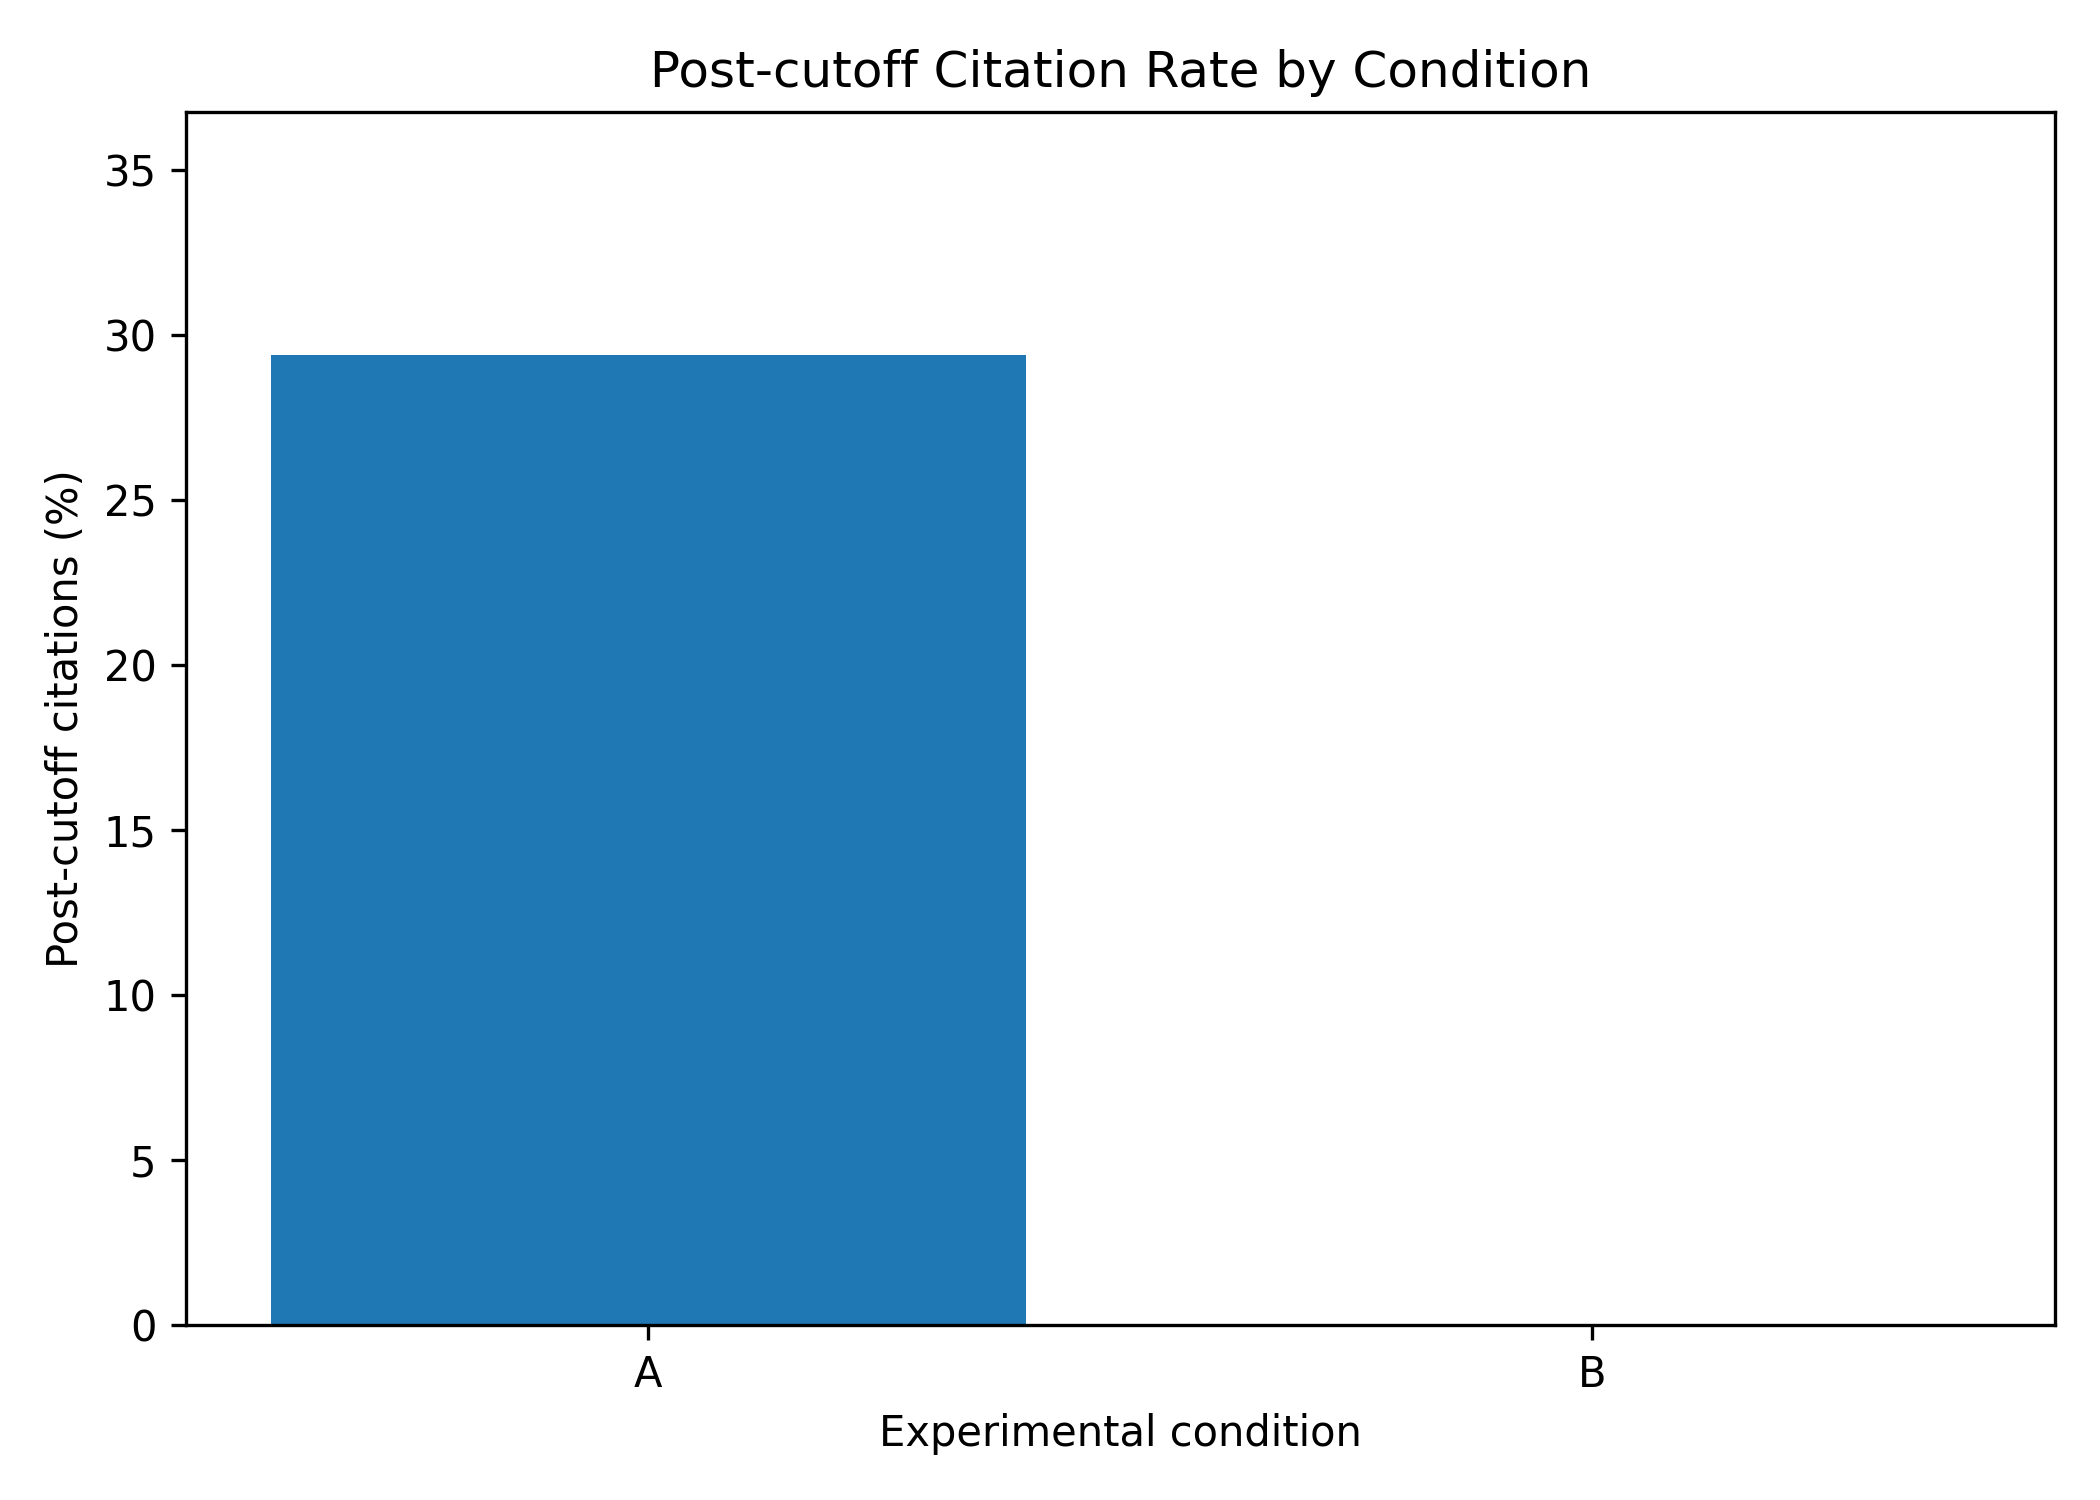
\includegraphics[width=.72\linewidth]{../results/figure1_overall_cutoff_rate.png}
\caption{Overall post-cutoff citation rates from the archived study analysis.}
\end{figure}

\subsection{Matched-pair comparison}
The pair-specific post-cutoff rates for A were 30.00\%, 30.00\%, 30.00\%, 18.18\%, and 40.00\%; all corresponding B rates were 0\%. The mean paired reduction was 29.64 percentage points. The exact two-sided sign test yielded $p=0.0625$, which does not meet the conventional $\alpha=0.05$ threshold.

\begin{figure}[h]
\centering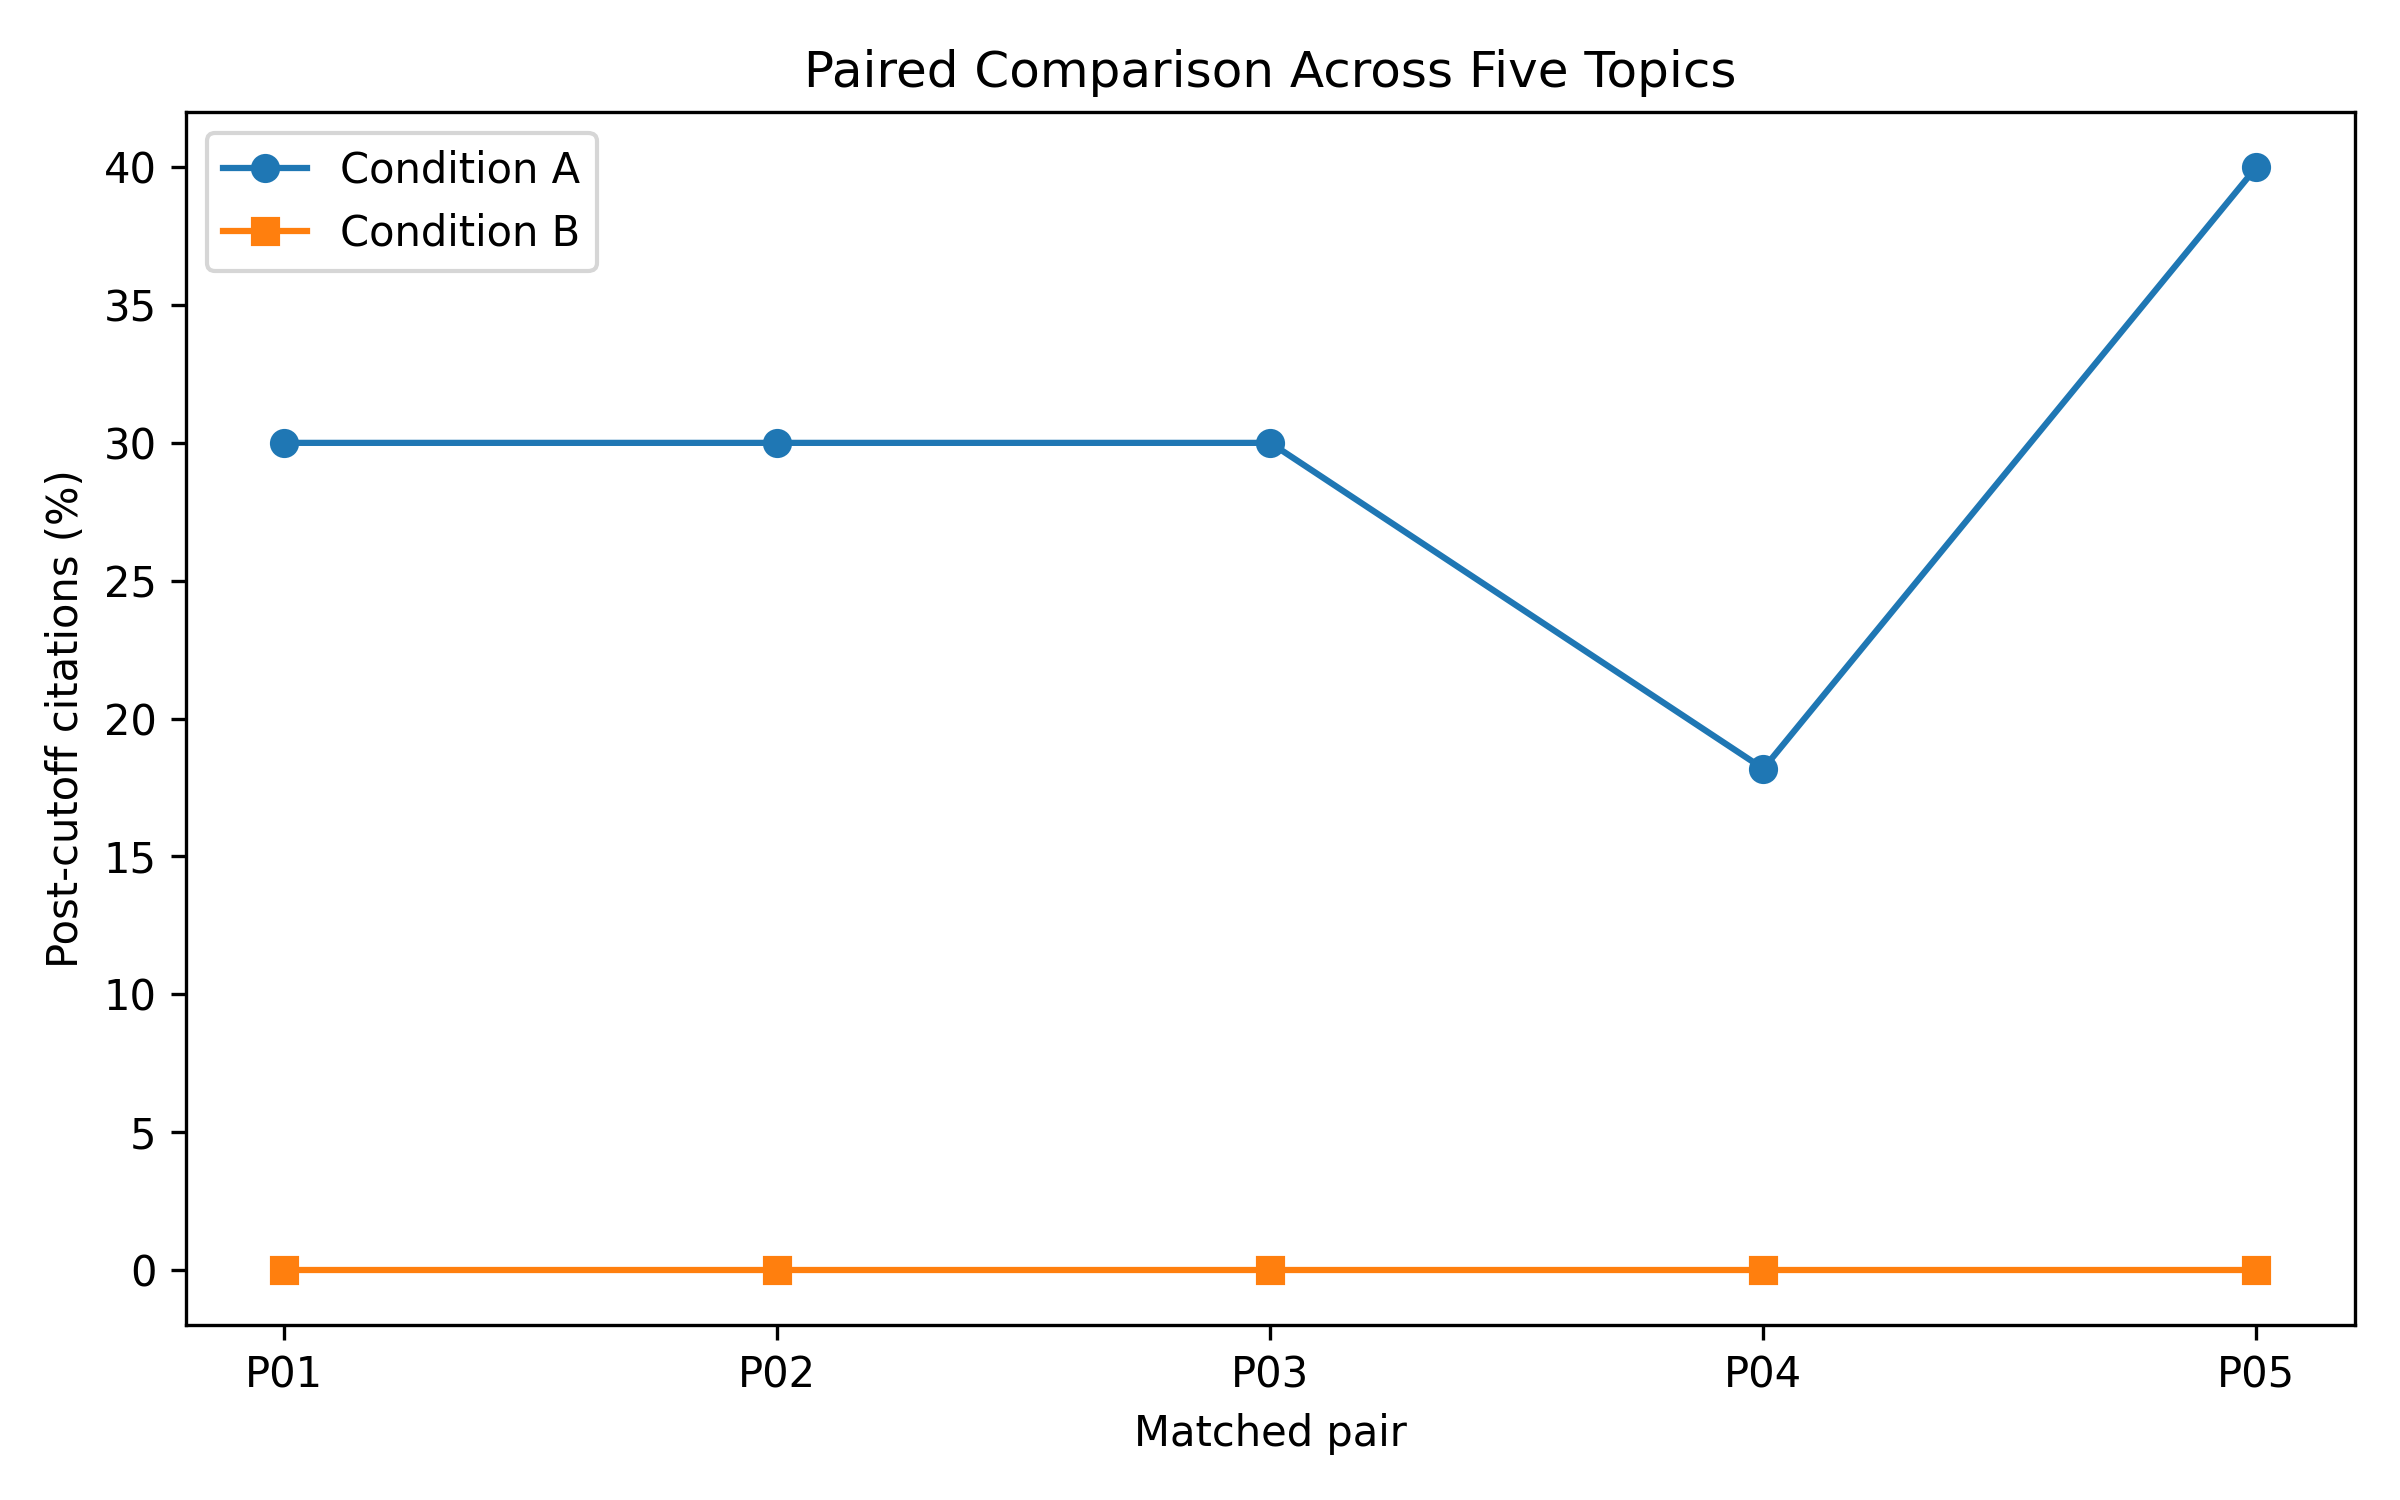
\includegraphics[width=.78\linewidth]{../results/figure2_paired_comparison.png}
\caption{Post-cutoff rates across five matched pairs.}
\end{figure}

\subsection{Bibliographic audit and sensitivity analysis}
The 100 extracted candidates comprised 93 MATCH, five PARTIAL\_MATCH, one DOI\_MISMATCH, and one NOT\_APPLICABLE entry. The NOT\_APPLICABLE item was excluded from the 99 analyzed references. Condition A had 45 MATCH entries among 51 (88.24\%); B had 48 among 48 (100\%). In the MATCH-only sensitivity analysis, A retained 12 post-cutoff references among 45 confirmed matches (26.67\%), while B retained none among 48. The mean paired reduction was 27.14 percentage points.

\begin{figure}[h]
\centering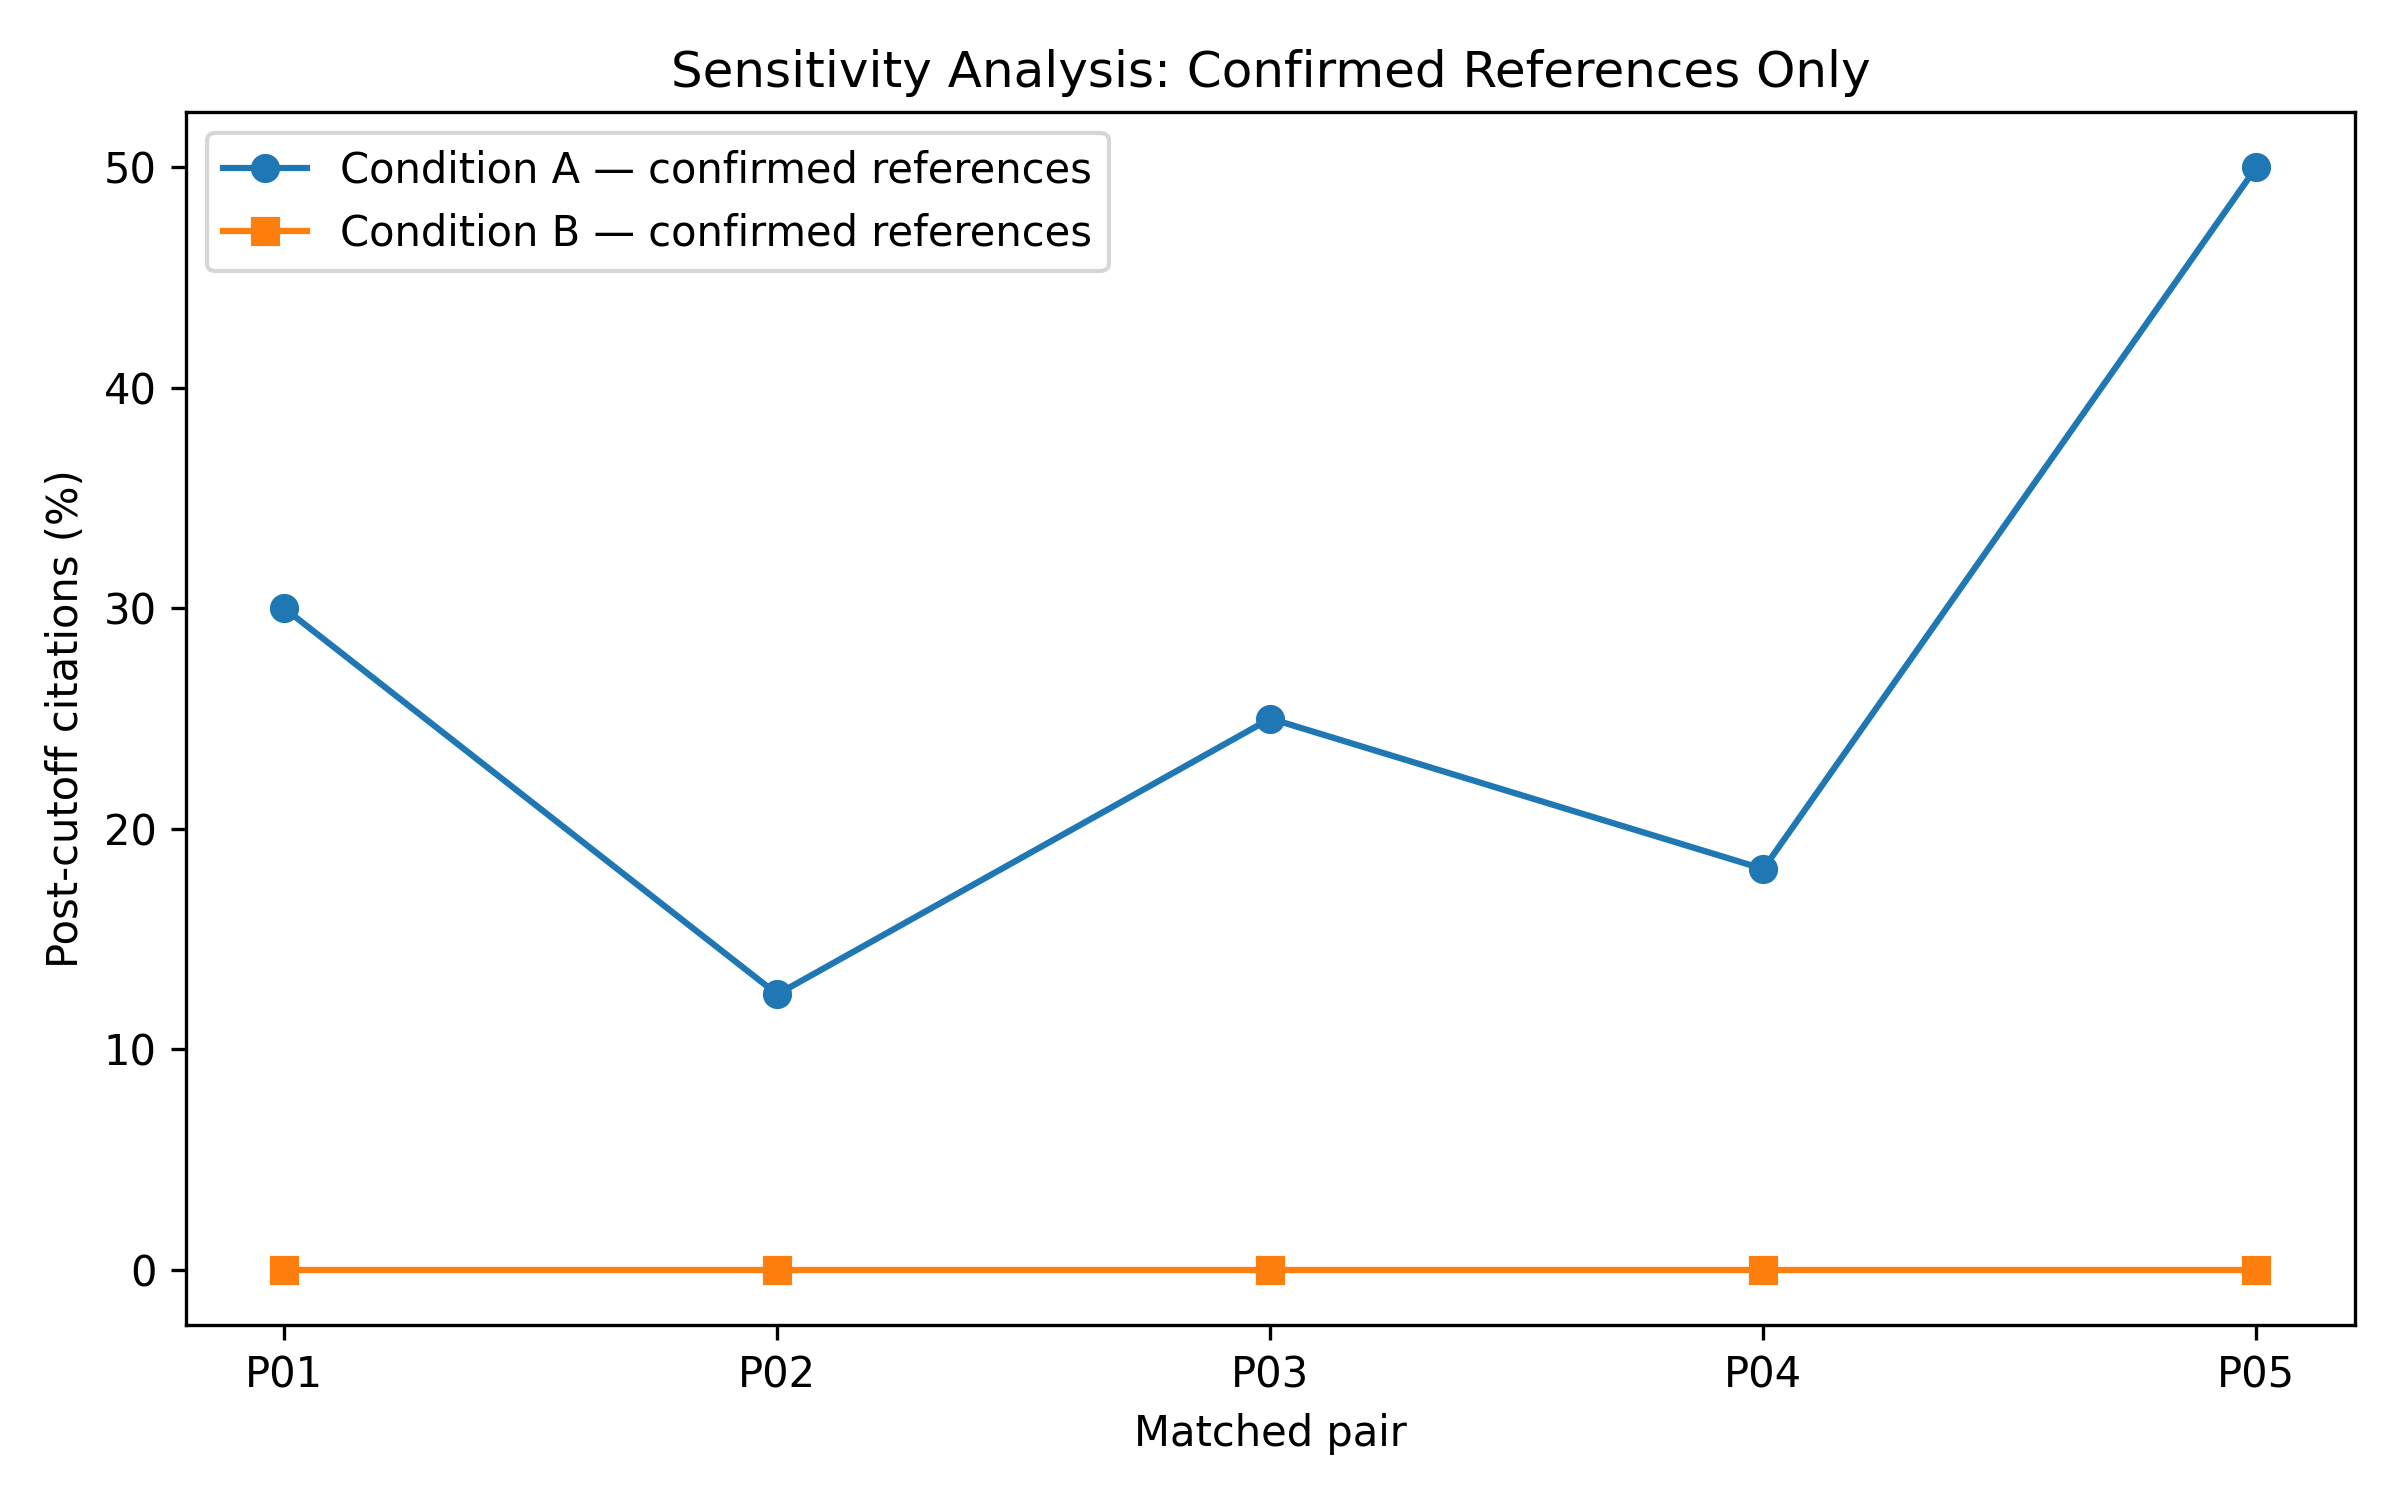
\includegraphics[width=.78\linewidth]{../results/figure3_sensitivity_analysis.png}
\caption{Sensitivity analysis restricted to bibliographically matched references.}
\end{figure}

\section{Discussion}
The observed results are consistent with the possibility that an explicit publication-date boundary instruction improves observable temporal compliance. The pattern was directionally consistent across all five pairs and remained in the MATCH-only sensitivity analysis. However, the small sample and non-significant exact sign test require cautious interpretation. The higher bibliographic match rate in B is an observed sample difference, not evidence that temporal instructions generally improve reference accuracy.

The experiment concerns compliance with a stated publication-date boundary. It does not reveal the model's internal training-data cutoff or the date on which it acquired particular information. The appearance of a post-cutoff citation could arise through context, retrieval, model updates, or other mechanisms; conversely, omission of a work does not prove lack of knowledge.

\section{Limitations}
The study contains only five matched pairs and uses one ChatGPT interface/model configuration, limiting statistical power and generalizability. The reviews exceeded the planned 800--1,000-word target; original outputs were retained and this deviation was not corrected after generation. Some bibliographic records remain partial or inconsistent. Publication-year classification can depend on whether the cited item is a preprint or later proceedings version. Manual UI generation is not a deterministic API reproduction. The archived CSV analysis script re-computes descriptive results but does not regenerate the original LLM outputs or independently validate every manual audit decision.

\section{Conclusion}
In this sample, Condition A produced a 29.41\% post-cutoff citation rate and Condition B produced 0\%. The mean paired reduction was 29.64 percentage points, while the exact two-sided sign test was $p=0.0625$. The MATCH-only sensitivity analysis retained a 27.14-point mean paired reduction. Explicit temporal instructions may be a useful practical control, but they do not replace independent bibliographic verification and do not measure a model's internal knowledge boundary. Larger studies across models, domains, and repeated generations are needed.

\section*{Reproducibility statement}
The repository includes ten generated review text files, extracted citation and audit CSVs, a prompt protocol, and a Python script for re-analysis of the archived tables. From the experiment directory, run \texttt{python scripts/reproduce\_analysis.py}. This command regenerates descriptive CSVs and figures under \texttt{results/reproduced/}; it does not reproduce the original manual ChatGPT generations.

\end{document}
